%============================================================
% Two-qubit quantum sensors (spin + spatial-mode entanglement)
% Graduate mini-course Beamer deck (ready to compile)
%
% Save as: two_qubit_sensor_observables.tex
% Compile: pdflatex two_qubit_sensor_observables.tex
%          (run twice for references)
% Or:      xelatex two_qubit_sensor_observables.tex
%
% Downloading / sharing: copy-paste into a .tex file; or host
% via Overleaf / GitHub / institutional repository; or email.
%============================================================

\documentclass[aspectratio=169]{beamer}

%============================================================
% Packages requested + practical
%============================================================
\usepackage{amsmath,amssymb,amsfonts}
\usepackage{physics} % requested (commutators, derivatives, etc.)

% ---- Resolve \bra/\ket command collisions between physics and braket ----
\let\bra\relax \let\ket\relax \let\braket\relax
\let\Bra\relax \let\Ket\relax \let\Braket\relax
\let\set\relax \let\Set\relax
\usepackage{braket}  % requested (Dirac notation)

\usepackage{bm}
\usepackage{quantikz} % requested (circuits)
\usepackage{booktabs}
\usepackage{multirow}
\usepackage{array}
\usepackage{siunitx}
\usepackage{tikz}
\usetikzlibrary{arrows.meta,positioning,calc}
\usepackage{pgfplots}
\pgfplotsset{compat=1.18}
\usepackage{listings}
\usepackage[round,authoryear]{natbib}

%============================================================
% Beamer styling
%============================================================
\usetheme{Madrid}
\setbeamertemplate{navigation symbols}{}
\setbeamertemplate{footline}[frame number]

%============================================================
% Listings (Python, optional Mermaid)
%============================================================
\lstset{
  basicstyle=\ttfamily\footnotesize,
  breaklines=true,
  columns=fullflexible,
  frame=single,
  showstringspaces=false
}

%============================================================
% Macros / notation
%============================================================
\newcommand{\Id}{\mathbb{I}}

\newcommand{\sA}[1]{\sigma_{#1}^{(A)}}
\newcommand{\sB}[1]{\sigma_{#1}^{(B)}}
\newcommand{\tA}[1]{\tau_{#1}^{(A)}}
\newcommand{\tB}[1]{\tau_{#1}^{(B)}}

\newcommand{\Jop}[1]{J_{#1}}
\newcommand{\Kop}[1]{K_{#1}}

\newcommand{\GcomS}{G_{\mathrm{com}}^{(s)}}
\newcommand{\GdiffS}{G_{\mathrm{diff}}^{(s)}}
\newcommand{\GcomM}{G_{\mathrm{com}}^{(m)}}
\newcommand{\GdiffM}{G_{\mathrm{diff}}^{(m)}}

\newcommand{\PiZs}{\Pi_{z}^{(s)}}
\newcommand{\PiZm}{\Pi_{z}^{(m)}}

\title[Two-qubit sensors: observables]{Observables for Two-Qubit Quantum Sensors with Spin and Spatial-Mode Entanglement}
\subtitle{Local, Nonlocal, and Hybrid Measurements; Metrology via (Q)FI; Connections to High-Energy Physics}
\author{Morten Hjorth-Jensen}
\date{March 10, 2026}

\begin{document}

%============================================================
\begin{frame}
  \titlepage
\end{frame}

%============================================================
\begin{frame}{Executive summary (what you will learn and use)}
\small
We study a \textbf{two-qubit quantum sensor prototype} where two subsystems $A,B$ each carry:
\begin{itemize}
\item a \textbf{spin qubit} (internal two-level system) and
\item a \textbf{spatial-mode qubit} (two-mode/path/position subspace),
\end{itemize}
on an \textbf{unspecified experimental platform}.

\vspace{0.35em}
This mini-course provides:
\begin{itemize}
\item A concrete \textbf{parameter-encoding} model (common-mode vs differential/gradient fields; spin, mode, and spin--mode couplings).
\item A structured set of \textbf{observable families} for diagnosing entanglement and sensing performance:
local, correlators, collective $J$ and $J^2$, rotated parity, Bell/CHSH, and hybrid spin--spatial observables.
\item A metrological bridge from observables to sensitivity using
\textbf{Cram\'er--Rao bounds}, \textbf{Fisher information}, and \textbf{QFI} (including $F_Q=4(\Delta G)^2$ for pure probes). \citep{BraunsteinCaves1994PRL,Paris2009IJQI,Pezze2018RMP}
\item \textbf{Measurement circuits} (Quantikz) for correlators, parity (direct and ancilla), and CHSH settings,
with compile-safe labels (math mode subscripts; \texttt{quantikz} not inside display math).
\item Worked examples (Bell, singlet/triplet, spatial Bell, common vs differential sensitivity with explicit QFI tables).
\item Experimental reality checks: dephasing, SPAM/readout, tomography vs direct measurement, shot-scaling.
\item Explicit mappings to \textbf{high-energy physics} (HEP) contexts: $t\bar t$ spin correlations, meson Bell tests,
detector models, neutrino/flavor qubits. \citep{BernreutherHeislerSi2015JHEP,BertlmannHiesmayr2001PRA,PeresTerno2004RMP,Banerjee2015EPJC,PozasKerstjensMartinMartinez2015PRD}
\end{itemize}
\end{frame}

%============================================================
\begin{frame}{Outline}
\small
\begin{itemize}
\item Physical setup and sensing generators (spin, spatial mode, hybrid).
\item Metrological framework: FI, QFI, Cram\'er--Rao; generator variances.
\item Observable families (definitions, what they probe, measurement circuits).
\item Worked examples: Bell states; singlet/triplet; spatial two-mode Bell; common vs differential fields.
\item Experimental considerations: dephasing, SPAM, tomography, shot budgets.
\item HEP connections and operator mappings.
\item Minimal measurement program + suggested experiments.
\item Python simulation (NumPy) for probes, encoding, dephasing, FI/QFI.
\end{itemize}
\end{frame}

%============================================================
\section{Physical setup}

%============================================================
\begin{frame}{Physical setup: two subsystems, spin + spatial-mode qubits}
\small
\textbf{Platform: unspecified.}
Interpret $A$ and $B$ as two addressable sensors (ions, atoms, NVs, superconducting qubits, etc.).

\vspace{0.35em}
Each subsystem $X\in\{A,B\}$ contains:
\begin{itemize}
\item \textbf{Spin qubit} Hilbert space $\mathcal{H}_{s,X}\cong\mathbb{C}^2$ with Pauli operators
$\sigma_x^{(X)},\sigma_y^{(X)},\sigma_z^{(X)}$.
\item \textbf{Spatial-mode qubit} Hilbert space $\mathcal{H}_{m,X}\cong\mathbb{C}^2$ with effective Pauli operators
$\tau_x^{(X)},\tau_y^{(X)},\tau_z^{(X)}$ (two paths/modes/locations).
\end{itemize}

Total Hilbert space:
\[
\mathcal{H}
=
(\mathcal{H}_{s,A}\otimes \mathcal{H}_{m,A})
\otimes
(\mathcal{H}_{s,B}\otimes \mathcal{H}_{m,B})
\cong
(\mathbb{C}^2)^{\otimes 4}.
\]

\vspace{0.25em}
\textbf{Entanglement structure:}
\begin{itemize}
\item Spin entanglement: across $\mathcal{H}_{s,A}\otimes\mathcal{H}_{s,B}$.
\item Mode entanglement: across $\mathcal{H}_{m,A}\otimes\mathcal{H}_{m,B}$.
\item Hybrid entanglement: involving spin and mode jointly (e.g., spin conditioned on mode).
\end{itemize}
\end{frame}

%============================================================
\begin{frame}{Parameter encoding: unitary model and generators}
\small
A sensing experiment encodes a parameter $\phi$ via
\[
\rho(\phi)=U(\phi)\,\rho_0\,U^\dagger(\phi),
\qquad
U(\phi)=e^{-i\phi G},
\]
where $G$ is the \textbf{generator} of the encoding. \citep{BraunsteinCaves1994PRL,Paris2009IJQI,Pezze2018RMP}

\vspace{0.35em}
We distinguish three broad sensing scenarios:
\begin{enumerate}
\item \textbf{Spin-only encoding:} $G$ built from $\sigma$ operators.
\item \textbf{Mode-only encoding:} $G$ built from $\tau$ operators (e.g., path potential differences).
\item \textbf{Hybrid encoding:} $G$ couples spin and mode (e.g., position-dependent Zeeman shifts).
\end{enumerate}

\vspace{0.35em}
Key theme:
\[
\textbf{Metrological relevance depends on }(\Delta G)^2\textbf{ for the chosen }G.
\]
Entanglement helps if it increases the variance of the \emph{right} generator.
\end{frame}

%============================================================
\begin{frame}{Common-mode vs differential (gradient) spin fields}
\small
A minimal spin-field interaction:
\[
H = \frac{\gamma}{2}\qty(B_A \sA{z} + B_B \sB{z}).
\]

Decompose
\[
B_A = B + \frac{\delta B}{2},
\qquad
B_B = B - \frac{\delta B}{2}.
\]
Then for evolution time $t$:
\[
U(t)=e^{-itH}
=
e^{-i\phi_{\mathrm{com}}\,\GcomS}\,
e^{-i\phi_{\mathrm{diff}}\,\GdiffS},
\]
with
\[
\GcomS=\frac{1}{2}(\sA{z}+\sB{z}),\quad
\GdiffS=\frac{1}{2}(\sA{z}-\sB{z}),
\quad
\phi_{\mathrm{com}}=\gamma B t,\quad
\phi_{\mathrm{diff}}=\gamma \frac{\delta B}{2}t.
\]

\vspace{0.35em}
Different entangled probes optimize different tasks:
\begin{itemize}
\item $\ket{\Phi}$-type (e.g., $\ket{\Phi^+}$) are sensitive to common-mode $\GcomS$.
\item $\ket{\Psi}$-type (e.g., $\ket{\Psi^+}$) are sensitive to differential $\GdiffS$.
\end{itemize}
\end{frame}

%============================================================
\begin{frame}{Mode-phase encoding (two-mode spatial qubit)}
\small
Let each mode qubit have basis $\ket{L}$ and $\ket{R}$, with
\[
\tau_z\ket{L}=+\ket{L},\qquad \tau_z\ket{R}=-\ket{R}.
\]
Then a spatial phase difference (e.g., potential imbalance between $L$ and $R$) can be modeled as
\[
H_m=\frac{\kappa}{2}\qty(V_A \tA{z}+V_B \tB{z})
\quad\Rightarrow\quad
U_m(t)=e^{-i\phi_m G_m}.
\]
Define
\[
\GcomM=\frac{1}{2}(\tA{z}+\tB{z}),\qquad
\GdiffM=\frac{1}{2}(\tA{z}-\tB{z})
\]
as common-mode and differential mode generators.

\vspace{0.35em}
\textbf{Parallelism to spin:} spatial Bell states can act as gradiometers for differential phases.
\end{frame}

%============================================================
\begin{frame}{Hybrid spin--mode encoding (position-dependent spin coupling)}
\small
If the field depends on spatial mode (e.g., opposite Zeeman shifts on two paths), a natural generator is
\[
G_{sz}
=
\frac{1}{2}\qty(\sA{z}\tA{z}+\sB{z}\tB{z}).
\]
This encodes a parameter $\phi$ via
\[
U(\phi)=\exp\qty[-i\phi G_{sz}].
\]

\vspace{0.35em}
\textbf{Consequences:}
\begin{itemize}
\item Spin-only measurements can be insufficient: the signal is stored in spin \emph{conditioned on mode}.
\item Hybrid observables like $\sA{z}\tA{z}$ and
$(\sA{z}\tA{z})(\sB{z}\tB{z})$
become the relevant diagnostics.
\end{itemize}
\end{frame}

%============================================================
\section{Metrological framework (FI/QFI)}

%============================================================
\begin{frame}{Classical Fisher information and Cram\'er--Rao bound}
\small
Given measurement outcomes $o$ with probabilities $p(o|\phi)$, the \textbf{classical Fisher information (FI)} is
\[
F_C(\phi)=\sum_o \frac{\qty(\partial_\phi p(o|\phi))^2}{p(o|\phi)}.
\]
For $\nu$ independent repetitions (shots), the Cram\'er--Rao bound:
\[
\mathrm{Var}(\hat\phi) \ge \frac{1}{\nu\,F_C(\phi)}.
\]
This is the operational link between \textbf{chosen observable/measurement} and achievable sensitivity. \citep{Paris2009IJQI}

\vspace{0.35em}
Binary outcome example ($o\in\{+,-\}$):
\[
F_C(\phi)=\frac{(\partial_\phi p_+)^2}{p_+}+\frac{(\partial_\phi p_-)^2}{p_-},\quad p_-=1-p_+.
\]
\end{frame}

%============================================================
\begin{frame}{Quantum Fisher information (QFI) and ultimate precision}
\small
The \textbf{quantum Fisher information (QFI)} is the maximum FI over all POVMs:
\[
F_Q(\phi)=\max_{\text{measurements}} F_C(\phi).
\]
For unitary encoding $\rho(\phi)=e^{-i\phi G}\rho_0 e^{i\phi G}$, $F_Q$ depends on $\rho_0$ and $G$. \citep{BraunsteinCaves1994PRL,Paris2009IJQI}

\vspace{0.35em}
\textbf{Pure probes} $\rho_0=\ket{\psi_0}\bra{\psi_0}$:
\[
\boxed{F_Q = 4(\Delta G)^2_{\psi_0}}.
\]
Thus, generator variance is the central metrological resource. \citep{Pezze2018RMP,Giovannetti2011NatPhoton}

\vspace{0.35em}
\textbf{Mixed probes:} the variance formula does not hold; one can use the spectral formula (next slide).
\end{frame}

%============================================================
\begin{frame}{QFI for mixed states under unitary encoding (spectral formula)}
\small
Let $\rho_0=\sum_i \lambda_i \ket{i}\bra{i}$ (eigendecomposition), and the encoding is generated by Hermitian $G$.
Then the QFI can be written as \citep{BraunsteinCaves1994PRL,Paris2009IJQI}
\[
F_Q(\rho_0,G)
=
2\sum_{i,j:\,\lambda_i+\lambda_j>0}
\frac{(\lambda_i-\lambda_j)^2}{\lambda_i+\lambda_j}\,
\abs{\bra{i}G\ket{j}}^2.
\]
For a pure state ($\lambda_0=1$), this reduces to $F_Q=4(\Delta G)^2$.

\vspace{0.35em}
\textbf{Practical use:}
this formula is what we will implement in the Python simulation for dephased (mixed) states.
\end{frame}

%============================================================
\begin{frame}{Entanglement and QFI benchmarks for linear generators}
\small
For $N$ qubits and a collective linear generator, separable states obey QFI bounds.
A common statement: for a linear two-mode interferometer, separable probes satisfy $F_Q \le N$. \citep{Hyllus2012PRA,Pezze2018RMP}

\vspace{0.35em}
For \textbf{two qubits} ($N=2$) and generators such as $\GcomS$ or $\GdiffS$:
\[
F_Q \le 2 \quad \text{for separable probes,}
\qquad
F_Q \le 4 \quad \text{(two-qubit ``Heisenberg'' maximum).}
\]
Thus $F_Q>2$ certifies entanglement that is useful for estimating the parameter encoded by that generator.

\vspace{0.35em}
\textbf{Caveat:}
Entanglement is \emph{task-dependent}. A state can be maximally entangled yet have $F_Q=0$ for some generators.
\end{frame}

%============================================================
\section{Observable families: definitions, meaning, measurement circuits}

%============================================================
\begin{frame}{Observable taxonomy (spin, mode, hybrid)}
\small
We use six observable families (spin forms shown; mode analogs via $\sigma\to\tau$):
\begin{enumerate}
\item \textbf{Local:} $\sA{\alpha}$, $\sB{\alpha}$.
\item \textbf{Two-body correlators:} $\sA{\alpha}\sB{\beta}$.
\item \textbf{Collective:} $\Jop{\alpha}=\frac12(\sA{\alpha}+\sB{\alpha})$ and moments $\Jop{\alpha}^2$.
\item \textbf{Parity (rotated parity):} $\PiZs=\sA{z}\sB{z}$ and $R^\dagger \PiZs R$.
\item \textbf{Bell/CHSH:} $\mathcal{B}_{\mathrm{CHSH}}$ built from correlators in rotated bases. \citep{CHSH1969PRL}
\item \textbf{Hybrid spin--mode:} $\sA{\alpha}\tA{\mu}$ and $(\sA{\alpha}\tA{\mu})(\sB{\beta}\tB{\nu})$.
\end{enumerate}

\vspace{0.35em}
\textbf{Metrology link:}
Many relevant generators are \emph{collective} or \emph{hybrid}; their variances are determined by correlators and parity-type observables. \citep{Pezze2018RMP}
\end{frame}

%============================================================
\subsection{Local observables}

%============================================================
\begin{frame}{Local observables: baseline diagnostics (often entanglement-blind)}
\small
\textbf{Spin local:}
\[
\expval{\sA{\alpha}},\qquad \expval{\sB{\alpha}},
\qquad \alpha\in\{x,y,z\}.
\]
\textbf{Mode local:}
\[
\expval{\tA{\mu}},\qquad \expval{\tB{\mu}},
\qquad \mu\in\{x,y,z\}.
\]

\vspace{0.35em}
\textbf{What they probe:}
direct coupling of the parameter to one subsystem, calibration (which qubit couples?), drift monitoring.

\vspace{0.35em}
\textbf{What they miss:}
For many entangled probes (all Bell states), all one-body marginals vanish:
\[
\expval{\sA{\alpha}}=\expval{\sB{\alpha}}=0\quad \forall\,\alpha.
\]
Hence local observables alone can fail to reveal the mechanism of entanglement-enhanced sensing.
\end{frame}

%============================================================
\subsection{Two-body correlators}

%============================================================
\begin{frame}{Two-body correlators: the primary ``whole-system'' observables}
\small
Define the spin correlation tensor
\[
C_{\alpha\beta}^{(s)}=\expval{\sA{\alpha}\sB{\beta}},
\qquad \alpha,\beta\in\{x,y,z\}.
\]
Similarly for spatial modes:
\[
C_{\mu\nu}^{(m)}=\expval{\tA{\mu}\tB{\nu}}.
\]

\vspace{0.35em}
\textbf{Connected correlators} remove product contributions:
\[
\expval{\sA{\alpha}\sB{\beta}}_c=
\expval{\sA{\alpha}\sB{\beta}}-\expval{\sA{\alpha}}\expval{\sB{\beta}}.
\]

\vspace{0.35em}
\textbf{Metrological content:}
Second moments of collective generators are fixed by correlators. Example:
\[
\Jop{z}=\frac12(\sA{z}+\sB{z}),
\quad
\Jop{z}^2
=
\frac12\Id + \frac12\sA{z}\sB{z}.
\]
Therefore $\expval{\sA{z}\sB{z}}$ directly determines $\expval{J_z^2}$ and helps determine $(\Delta J_z)^2$ and thus QFI for common-mode sensing. \citep{Pezze2018RMP}
\end{frame}

%============================================================
\begin{frame}{Measuring a Pauli string: basis-change principle}
\small
Most observables reduce to Pauli strings. Measure $\expval{P}$ where
\[
P=\bigotimes_{k=1}^n P_k,\quad P_k\in\{X,Y,Z\}.
\]
Procedure:
\begin{enumerate}
\item Apply a local unitary $U_k$ to map $P_k$ to $Z$:
\[
X=H Z H,\qquad
Y=(HS^\dagger) Z (S H).
\]
\item Measure all qubits in $Z$.
\item Multiply outcomes to estimate $\expval{P}$.
\end{enumerate}

\vspace{0.35em}
This is the standard measurement primitive used in VQE, tomography, and correlator estimation. \citep{Kay2018Quantikz}
\end{frame}

%============================================================
\begin{frame}{Circuit sketch: measuring $\expval{\sA{x}\sB{y}}$ (example)}
\small
Goal: estimate $\expval{X_A Y_B}$.

\vspace{0.3em}
\begin{center}
\begin{quantikz}[row sep=0.25cm, column sep=0.4cm]
\lstick{$q_A$} & \gate{H} & \meter{} \\
\lstick{$q_B$} & \gate{S^\dagger} & \gate{H} & \meter{}
\end{quantikz}
\end{center}

\vspace{0.3em}
If measurement outcomes are mapped to $\pm 1$ values $m_A,m_B$, then for $\nu$ shots:
\[
\widehat{\expval{X_A Y_B}}=\frac{1}{\nu}\sum_{k=1}^{\nu} m_A^{(k)}m_B^{(k)}.
\]
\end{frame}

%============================================================
\begin{frame}{Correlator estimation from counts (explicit formula)}
\small
For two-qubit dichotomic outcomes $(m_A,m_B)\in\{\pm 1\}^2$,
counts $N_{++},N_{+-},N_{-+},N_{--}$ yield
\[
\widehat{E}
=
\widehat{\expval{A\otimes B}}
=
\frac{N_{++}+N_{--}-N_{+-}-N_{-+}}{N_{\mathrm{tot}}}.
\]

\vspace{0.35em}
\textbf{Shot scaling (binomial / bounded outcomes):}
\[
\mathrm{Var}(\widehat{E})\approx \frac{1-E^2}{\nu}\le \frac{1}{\nu},
\]
so additive error $\epsilon$ typically costs $\nu=\mathcal{O}(\epsilon^{-2})$ shots per setting.

\vspace{0.35em}
Importance: measurement setting count $\times$ $\epsilon^{-2}$ dominates budgets, motivating direct measurement (few settings) over full tomography when possible.
\end{frame}

%============================================================
\subsection{Collective observables}

%============================================================
\begin{frame}{Collective spin observables: $J$ and $J^2$}
\small
Define collective spin operators:
\[
\Jop{\alpha}=\frac12(\sA{\alpha}+\sB{\alpha}),
\qquad \alpha\in\{x,y,z\}.
\]
Second moments:
\[
\Jop{\alpha}^2
=
\frac12\Id + \frac12\sA{\alpha}\sB{\alpha}.
\]
Thus measuring $\expval{\sA{\alpha}\sB{\alpha}}$ gives $\expval{J_\alpha^2}$.

\vspace{0.35em}
For pure probes and unitary encoding generated by $\Jop{z}$:
\[
F_Q = 4(\Delta \Jop{z})^2.
\]
Hence collective fluctuations are directly metrological. \citep{Pezze2018RMP,Giovannetti2011NatPhoton}

\vspace{0.35em}
Mode collective operators are analogous:
\[
\Kop{\mu}=\frac12(\tA{\mu}+\tB{\mu}).
\]
\end{frame}

%============================================================
\begin{frame}{Total spin $\mathbf{J}^2$ and singlet/triplet discrimination}
\small
Define
\[
\mathbf{J}^2=\Jop{x}^2+\Jop{y}^2+\Jop{z}^2
=
\frac{3}{2}\Id+\frac12\qty(\sA{x}\sB{x}+\sA{y}\sB{y}+\sA{z}\sB{z}).
\]
Eigenvalues:
\[
\mathbf{J}^2\ket{j,m}=j(j+1)\ket{j,m}
\quad\Rightarrow\quad
j=1:\mathbf{J}^2=2,\;\;j=0:\mathbf{J}^2=0.
\]

\vspace{0.35em}
\textbf{Measurement:} estimate $XX$, $YY$, $ZZ$ correlators and combine linearly to obtain $\expval{\mathbf{J}^2}$.

\vspace{0.35em}
\textbf{Sensing relevance:}
singlet ($j=0$) is immune to common-mode generators like $\Jop{z}$, while triplets respond.
This is important for common-mode rejection vs gradient sensing.
\end{frame}

%============================================================
\subsection{Parity observables}

%============================================================
\begin{frame}{Parity: definition and rotated parity readout}
\small
Spin $z$-parity:
\[
\PiZs=\sA{z}\sB{z}\in\{+1,-1\}.
\]
Mode parity similarly:
\[
\PiZm=\tA{z}\tB{z}.
\]

\vspace{0.35em}
\textbf{Rotated parity:}
apply a (possibly collective) rotation $R(\theta)$ then measure $z$-parity:
\[
\Pi^{(s)}(\theta)=R^\dagger(\theta)\,\PiZs\,R(\theta).
\]
For example, measuring $X$-parity is just Hadamards before $Z$ readout:
\[
X\text{-parity }=\sA{x}\sB{x}=(H\otimes H)\,\PiZs\,(H\otimes H).
\]

\vspace{0.35em}
Parity measurements are widely used as high-contrast interferometric readout observables, often approaching optimality for certain nonclassical probes. \citep{Gerry2010Parity,Pezze2018RMP}
\end{frame}

%============================================================
\begin{frame}{Parity measurement I: direct (no ancilla)}
\small
Measure both qubits in $Z$ and post-process:
\[
\PiZs = m_A m_B, \qquad m_A,m_B\in\{\pm 1\}.
\]

\vspace{0.3em}
\begin{center}
\begin{quantikz}[row sep=0.25cm, column sep=0.6cm]
\lstick{$q_A$} & \meter{} \\
\lstick{$q_B$} & \meter{}
\end{quantikz}
\end{center}

\vspace{0.25em}
Rotated parity: insert basis changes (e.g., $H$ or $S^\dagger H$ gates) before measurement.
This becomes a Pauli-string measurement of $XX$, $YY$, etc.
\end{frame}

%============================================================
\begin{frame}{Parity measurement II: ancilla-based parity mapping}
\small
If hardware favors reading out one qubit, map parity to an ancilla $a$:

\vspace{0.25em}
\begin{center}
\begin{quantikz}[row sep=0.25cm, column sep=0.35cm]
\lstick{$q_A$} & \ctrl{2} & \qw \\
\lstick{$q_B$} & \qw      & \ctrl{1} & \qw \\
\lstick{$a$}   & \targ{}  & \targ{}  & \meter{}
\end{quantikz}
\end{center}

\vspace{0.25em}
Initialize $a$ in $\ket{0}$:
the ancilla measurement outcome satisfies $m_a=m_A m_B$, i.e.\ it returns parity.
For $X$- or $Y$-parity, apply basis changes on $q_A,q_B$ before the CNOT ladder.
\end{frame}

%============================================================
\subsection{Bell/CHSH observables}

%============================================================
\begin{frame}{Bell/CHSH operator (built from correlators)}
\small
Choose dichotomic observables (outcomes $\pm 1$)
\[
A_0,A_1\text{ on }A;\qquad B_0,B_1\text{ on }B.
\]
CHSH Bell operator:
\[
\mathcal{B}_{\mathrm{CHSH}}
=
A_0\otimes(B_0+B_1)+A_1\otimes(B_0-B_1).
\]
Define correlators $E_{xy}=\expval{A_x\otimes B_y}$, then
\[
S=E_{00}+E_{01}+E_{10}-E_{11}=\expval{\mathcal{B}_{\mathrm{CHSH}}}.
\]
Local hidden-variable theories imply $|S|\le 2$; quantum mechanics allows $|S|\le 2\sqrt2$. \citep{CHSH1969PRL}

\vspace{0.35em}
\textbf{Sensing relevance:}
CHSH is not a phase estimator per se, but it is a compact diagnostic of nonlocal correlation quality (useful under noise/SPAM and for validating entanglement resources used in sensing).
\end{frame}

%============================================================
\begin{frame}{Canonical CHSH measurement settings and basis rotations}
\small
A standard choice that maximally violates CHSH on $\ket{\Phi^+}$ is
\[
A_0=Z,\quad A_1=X,
\qquad
B_0=\frac{Z+X}{\sqrt2},\quad B_1=\frac{Z-X}{\sqrt2}.
\]
Realize $B_0,B_1$ by single-qubit rotations on $B$:
\[
B_0 = R_y(-\tfrac{\pi}{4})\,Z\,R_y(\tfrac{\pi}{4}),
\qquad
B_1 = R_y(\tfrac{\pi}{4})\,Z\,R_y(-\tfrac{\pi}{4}).
\]
Thus each correlator is a $Z\otimes Z$ measurement in an appropriate rotated basis.

\vspace{0.35em}
Computing $S$ requires four settings ($E_{00},E_{01},E_{10},E_{11}$).
\end{frame}

%============================================================
\begin{frame}{Circuit sketch: measuring one CHSH correlator $E_{00}$}
\small
Example: $E_{00}=\expval{A_0\otimes B_0}=\expval{Z\otimes (Z+X)/\sqrt2}$.

\vspace{0.3em}
\begin{center}
\begin{quantikz}[row sep=0.25cm, column sep=0.5cm]
\lstick{$q_A$} & \qw & \meter{} \\
\lstick{$q_B$} & \gate{R_y(-\pi/4)} & \meter{}
\end{quantikz}
\end{center}

\vspace{0.25em}
Then compute $\widehat{E}_{00}$ from the $\pm 1$ outcomes and repeat for the other three settings.
\end{frame}

%============================================================
\subsection{Hybrid spin--spatial observables}

%============================================================
\begin{frame}{Hybrid spin--mode observables (essential for position-dependent sensing)}
\small
Define local hybrid operators:
\[
O_A^{(sz)}=\sA{z}\tA{z},
\qquad
O_B^{(sz)}=\sB{z}\tB{z}.
\]
Two-system hybrid correlators:
\[
C_{\alpha\mu,\beta\nu}^{(sm)}
=
\expval{(\sA{\alpha}\tA{\mu})(\sB{\beta}\tB{\nu})}.
\]
Hybrid parity-like string:
\[
\Pi_{zz}^{(sm)}=(\sA{z}\tA{z})(\sB{z}\tB{z}).
\]

\vspace{0.35em}
\textbf{Metrological necessity:}
If encoding generator is $G_{sz}=\frac12(\sA{z}\tA{z}+\sB{z}\tB{z})$, then
\[
F_Q(\text{pure})=4(\Delta G_{sz})^2
\]
depends on hybrid correlators and cannot, in general, be inferred from spin-only measurements.

\vspace{0.35em}
\textbf{Measurement:}
treat spin and mode qubits as four physical qubits and measure the corresponding Pauli string via basis changes and $Z$ readout.
\end{frame}

%============================================================
\begin{frame}{Circuit sketch: measuring a hybrid Pauli string (example)}
\small
Example hybrid observable:
\[
P=(\sA{x}\tA{z})(\sB{y}\tB{x})
\quad\text{(a Pauli string on four qubits).}
\]
Assume qubit ordering: $(s_A,m_A,s_B,m_B)$.

\vspace{0.25em}
\begin{center}
\begin{quantikz}[row sep=0.22cm, column sep=0.32cm]
\lstick{$s_A$} & \gate{H} & \meter{} \\
\lstick{$m_A$} & \qw      & \meter{} \\
\lstick{$s_B$} & \gate{S^\dagger} & \gate{H} & \meter{} \\
\lstick{$m_B$} & \gate{H} & \meter{}
\end{quantikz}
\end{center}

\vspace{0.25em}
Post-process by multiplying all four $\pm 1$ outcomes to estimate $\expval{P}$.
\end{frame}

%============================================================
\section{Worked examples (expectation values, QFI, common vs differential)}

%============================================================
\begin{frame}{Worked example 1: Bell states (spin) and correlator signatures}
\small
Bell states:
\[
\ket{\Phi^\pm}=\frac{1}{\sqrt2}(\ket{00}\pm\ket{11}),
\qquad
\ket{\Psi^\pm}=\frac{1}{\sqrt2}(\ket{01}\pm\ket{10}).
\]
All one-body marginals vanish: $\expval{\sA{\alpha}}=\expval{\sB{\alpha}}=0$.

\vspace{0.35em}
Key correlators (spin):
\[
\expval{XX},\ \expval{YY},\ \expval{ZZ}.
\]

\begin{center}
\small
\begin{tabular}{lccc}
\toprule
State & $\expval{\sA{x}\sB{x}}$ & $\expval{\sA{y}\sB{y}}$ & $\expval{\sA{z}\sB{z}}$ \\
\midrule
$\ket{\Phi^+}$ & $+1$ & $-1$ & $+1$ \\
$\ket{\Phi^-}$ & $-1$ & $+1$ & $+1$ \\
$\ket{\Psi^+}$ & $+1$ & $+1$ & $-1$ \\
$\ket{\Psi^-}$ (singlet) & $-1$ & $-1$ & $-1$ \\
\bottomrule
\end{tabular}
\end{center}

\vspace{0.25em}
Thus Bell states are best identified and monitored via correlators/parity, not local means.
\end{frame}

%============================================================
\begin{frame}{Worked example 2: explicit QFI for common-mode vs differential encoding (spin)}
\small
Generators:
\[
\GcomS=\frac12(\sA{z}+\sB{z}),
\qquad
\GdiffS=\frac12(\sA{z}-\sB{z}).
\]
For pure probes, $F_Q=4(\Delta G)^2$.

\vspace{0.35em}
\begin{center}
\small
\begin{tabular}{lcc}
\toprule
Probe & $F_Q$ for $\GcomS$ (common) & $F_Q$ for $\GdiffS$ (diff) \\
\midrule
$\ket{+}\ket{+}$ & $2$ & $2$ \\
$\ket{\Phi^+}$ & $4$ & $0$ \\
$\ket{\Psi^+}$ & $0$ & $4$ \\
$\ket{\Psi^-}$ (singlet) & $0$ & $4$ \\
\bottomrule
\end{tabular}
\end{center}

\vspace{0.25em}
Interpretation:
\begin{itemize}
\item $\ket{\Phi^+}$ is an optimal two-qubit probe for common-mode $Z$ phase (Heisenberg-like factor $2$ in phase).
\item $\ket{\Psi^+}$ or $\ket{\Psi^-}$ are optimal for gradients/differentials.
\end{itemize}
\end{frame}

%============================================================
\begin{frame}{Worked example 3: singlet/triplet sensors (symmetry and immunity)}
\small
Triplet states:
\[
\ket{T_+}=\ket{00},\quad \ket{T_0}=\frac{1}{\sqrt2}(\ket{01}+\ket{10}),\quad \ket{T_-}=\ket{11},
\]
Singlet:
\[
\ket{S}=\ket{\Psi^-}=\frac{1}{\sqrt2}(\ket{01}-\ket{10}).
\]
Total spin:
\[
\mathbf{J}^2\ket{T_m}=2\ket{T_m},\qquad \mathbf{J}^2\ket{S}=0.
\]

\vspace{0.35em}
\textbf{Common-mode field ($\GcomS \propto \Jop{z}$):}
\[
\GcomS \ket{S}=0 \quad\Rightarrow\quad (\Delta \GcomS)^2=0 \Rightarrow F_Q=0.
\]
Thus the singlet is a \textbf{common-mode rejector}.

\vspace{0.35em}
\textbf{Differential field ($\GdiffS$):}
acts within the $\{\ket{01},\ket{10}\}$ subspace and generates relative phases; $\ket{T_0}$ and $\ket{S}$ are gradient-sensitive probes.
\end{frame}

%============================================================
\begin{frame}{Worked example 4: spatial (mode) Bell state as a gradiometer}
\small
Mode basis $\ket{L},\ket{R}$ with $\tau_z\ket{L}=+\ket{L}$ and $\tau_z\ket{R}=-\ket{R}$.

Spatial Bell-like state:
\[
\ket{\Psi_m^+}=\frac{1}{\sqrt2}\qty(\ket{L_A R_B}+\ket{R_A L_B}).
\]
Then (mode correlators):
\[
\expval{\tA{z}\tB{z}}=-1,\qquad
\expval{\tA{x}\tB{x}}=+1,\qquad
\expval{\tA{y}\tB{y}}=+1.
\]

\vspace{0.35em}
Mode generators:
\[
\GcomM=\frac12(\tA{z}+\tB{z}),\qquad
\GdiffM=\frac12(\tA{z}-\tB{z}).
\]
For $\ket{\Psi_m^+}$:
\[
F_Q(\ket{\Psi_m^+},\GcomM)=0,\qquad
F_Q(\ket{\Psi_m^+},\GdiffM)=4.
\]
So spatial entanglement naturally realizes a \textbf{two-mode gradiometer}.
\end{frame}

%============================================================
\begin{frame}{Worked example 5: rotated parity fringes for $\ket{\Phi^+}$ under common-mode encoding}
\small
Prepare $\ket{\Phi^+}=(\ket{00}+\ket{11})/\sqrt2$ and encode via $U(\phi)=e^{-i\phi \GcomS}$.
Up to a global phase:
\[
\ket{\psi(\phi)}=\frac{1}{\sqrt2}\qty(\ket{00}+e^{i2\phi}\ket{11}).
\]
Then
\[
\expval{\sA{x}\sB{x}} = \cos(2\phi),\qquad
\expval{\sA{y}\sB{y}} = -\cos(2\phi).
\]

\vspace{0.35em}
\textbf{Parity-as-correlator readout:}
Measure $XX$ by applying Hadamards and measuring $ZZ$ parity:
\[
\expval{XX}=\expval{(H\otimes H)\,\PiZs\,(H\otimes H)}.
\]
This yields fringes with doubled phase frequency (slope enhancement), consistent with $F_Q=4$.

\vspace{0.25em}
This is a prototypical demonstration of how a whole-system observable (correlator/parity) accesses entanglement-enhanced phase encoding.
\end{frame}

%============================================================
\section{Comparison tables and a QFI chart}

%============================================================
\begin{frame}{Comparison table: observables vs sensing targets and metrology}
\scriptsize
\renewcommand{\arraystretch}{1.2}
\begin{center}
\begin{tabular}{>{\raggedright\arraybackslash}p{2.85cm}
                >{\raggedright\arraybackslash}p{3.2cm}
                >{\raggedright\arraybackslash}p{3.3cm}
                >{\raggedright\arraybackslash}p{4.0cm}}
\toprule
\textbf{Observable} & \textbf{What it measures} &
\textbf{Common vs diff sensitivity} &
\textbf{Entanglement / QFI relevance} \\
\midrule
Local $\sA{\alpha}$ (or $\tA{\mu}$) & Single-subsystem polarization/occupation & Sensitive to local couplings; can miss global encoding & Often blind to entanglement; insufficient to certify metrological gain \\
Two-body $\sA{\alpha}\sB{\beta}$ & Correlation tensor component & Separates $\ket{\Phi}$-type (common) vs $\ket{\Psi}$-type (diff) tasks & Determines second moments of $\Jop{\alpha}$; feeds $(\Delta G)^2$ and thus QFI \\
Collective $\Jop{\alpha},\Jop{\alpha}^2$ & Global magnetization + fluctuations & Directly aligned with common-mode generators ($\GcomS$) & For pure probes: $F_Q=4(\Delta \Jop{\alpha})^2$ \\
Parity $\Pi^{(s)}(\theta)$ & Even/odd outcomes after readout rotation & High-contrast readout for phase fringes; works for both common/diff with correct rotation & Often near-optimal (state-dependent); relates to Pauli-string expectations \\
Bell/CHSH $S$ & Scalar summary of multiple correlators & Not a phase estimator but diagnoses nonlocal correlations under noise & Tracks entanglement quality; useful validation tool for sensing resources \\
Hybrid $\sA{z}\tA{z}$, etc. & Spin conditioned on mode; joint spin--mode correlations & Essential if encoding is mode-dependent or hybrid ($G_{sz}$) & Governs $(\Delta G)^2$ for hybrid generators; can reveal hybrid entanglement useful for sensing \\
\bottomrule
\end{tabular}
\end{center}
\end{frame}

%============================================================
\begin{frame}{Noise-limited metrology: QFI under dephasing (two-qubit illustration)}
\small
Independent dephasing is a canonical noise model for sensors (e.g., frequency standards).
It can destroy entanglement advantage beyond a crossover time. \citep{Huelga1997PRL,Demkowicz2015ProgOpt,Pezze2018RMP}

\vspace{0.25em}
Let $\eta=e^{-\Gamma t}$ denote single-qubit coherence.
A simple illustrative scaling for common-mode sensing:
\[
F_Q^{(\mathrm{prod})}\approx 2\eta^2,\qquad
F_Q^{(\Phi^+)}\approx 4\eta^4.
\]
Entangled probes can be best near $\eta\simeq 1$, but degrade faster under uncorrelated dephasing. \citep{Huelga1997PRL}

\vspace{0.2em}
\begin{center}
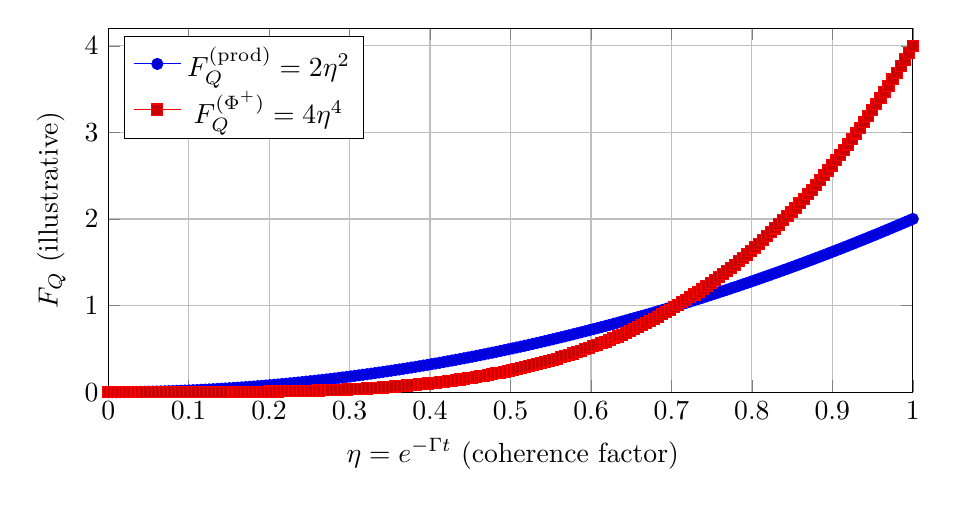
\begin{tikzpicture}
\begin{axis}[
  width=11.8cm,
  height=6.2cm,
  xlabel={$\,\eta=e^{-\Gamma t}$ (coherence factor)},
  ylabel={$F_Q$ (illustrative)},
  xmin=0, xmax=1,
  ymin=0, ymax=4.2,
  grid=both,
  legend style={at={(0.02,0.98)},anchor=north west,fill=white,draw=black},
]
\addplot+[domain=0:1, samples=200] {2*x^2};
\addlegendentry{$F_Q^{(\mathrm{prod})}=2\eta^2$}
\addplot+[domain=0:1, samples=200] {4*x^4};
\addlegendentry{$F_Q^{(\Phi^+)}=4\eta^4$}
\end{axis}
\end{tikzpicture}
\end{center}
\end{frame}

%============================================================
\section{Experimental considerations}

%============================================================
\begin{frame}{Dephasing channel model (Kraus form) and impact on observables}
\small
A common single-qubit dephasing (phase-flip) channel:
\[
\mathcal{E}_p(\rho)=(1-p)\rho + p\,Z\rho Z,
\]
with Kraus operators $K_0=\sqrt{1-p}\,\Id$, $K_1=\sqrt{p}\,Z$.

\vspace{0.35em}
Two-qubit independent dephasing:
\[
\rho \mapsto (\mathcal{E}_p\otimes \mathcal{E}_p)(\rho).
\]

\vspace{0.35em}
\textbf{Observable effects:}
\begin{itemize}
\item Coherences (and thus $XX$, $YY$, rotated parity fringes, CHSH) decay with $p$.
\item $ZZ$ parity may remain robust if populations are unchanged.
\item QFI and FI decrease; entanglement advantage can vanish. \citep{Huelga1997PRL,Demkowicz2015ProgOpt}
\end{itemize}
\end{frame}

%============================================================
\begin{frame}{Readout/SPAM errors and mitigation (platform unspecified)}
\small
Readout (SPAM) errors bias correlators and parity because they depend on products of outcomes.

\vspace{0.35em}
Typical mitigation approaches (platform-dependent):
\begin{itemize}
\item Calibrate a \textbf{confusion matrix} $M$ for outcome flips and invert/regularize classically.
\item Use measurement symmetrization / randomized compiling to average coherent readout bias.
\item Prefer a \textbf{minimal measurement program} tailored to the sensing generator to reduce the number of settings and accumulation of bias.
\end{itemize}

\vspace{0.35em}
Because the physical platform is unspecified, we do not assume a particular mitigation pipeline;
instead, we emphasize robust measurement choices (parity/correlators) plus calibration.
\end{frame}

%============================================================
\begin{frame}{Tomography vs direct measurement (settings and shot cost)}
\small
Two-qubit state tomography requires up to $15$ nontrivial Pauli expectations (excluding $\Id\otimes\Id$), usually grouped into a few local bases.

\vspace{0.35em}
\textbf{For sensing: direct measurement is usually better}:
\begin{itemize}
\item If theory predicts a generator $G$ and an (approx.) optimal measurement, measure only what you need:
$\expval{P}$ for a small set of Pauli strings $P$ that determine
$F_C$ or validate preparation.
\item Example common-mode sensing with $\ket{\Phi^+}$:
measure $XX$ (via rotated parity) plus $ZZ$ (parity) and optionally CHSH for entanglement validation.
\end{itemize}

\vspace{0.35em}
\textbf{Shot scaling:} additive error $\epsilon$ per setting typically costs $\nu=\mathcal{O}(\epsilon^{-2})$ shots.
Total cost scales roughly as $(\#\text{settings})/\epsilon^2$.
\end{frame}

%============================================================
\section{High-energy physics (HEP) connections and operator mappings}

%============================================================
\begin{frame}{HEP mapping I: spin density matrices and correlation tensors in $t\bar t$}
\small
In HEP, two-particle spin states are often described by a $4\times 4$ density matrix decomposed as
\[
\rho
=
\frac14\qty(
\Id\otimes\Id
+\sum_i B_i\,\sigma_i\otimes\Id
+\sum_j \bar B_j\,\Id\otimes\sigma_j
+\sum_{ij} C_{ij}\,\sigma_i\otimes\sigma_j
).
\]
Here $C_{ij}$ is the \textbf{spin correlation matrix}.

\vspace{0.35em}
\textbf{Direct mapping to sensor correlators:}
\[
C_{ij}\quad \longleftrightarrow\quad \expval{\sA{i}\sB{j}}.
\]
In top-pair physics, $C_{ij}$ is accessed via angular distributions of decay products, effectively implementing local spin measurements. \citep{BernreutherHeislerSi2015JHEP}

\vspace{0.35em}
Thus the same correlators used in quantum sensing diagnostics are canonical in HEP spin-correlation measurements.
\end{frame}

%============================================================
\begin{frame}{HEP mapping II: Bell tests with neutral mesons (kaons, $B$ mesons)}
\small
Neutral meson pairs (e.g., $K^0\bar K^0$) form entangled ``quasi-spin'' systems. \citep{BertlmannHiesmayr2001PRA}

\vspace{0.25em}
\textbf{Operator mapping idea:}
Choose a two-level basis, e.g.
\[
\ket{K^0}\equiv\ket{0},\qquad \ket{\bar K^0}\equiv\ket{1}.
\]
Then strangeness measurement corresponds to a Pauli-$Z$-type observable on quasi-spin:
\[
S \sim \sigma_z.
\]
Other measurement choices (CP eigenstates, different decay channels, or time-tagged measurements) correspond to rotated Pauli axes, enabling Bell-type inequalities.

\vspace{0.35em}
\textbf{Analogy to sensing:}
multiple correlator settings (CHSH) are measured in different bases/times, similar to rotating measurement bases in two-qubit sensors.
\end{frame}

%============================================================
\begin{frame}{HEP mapping III: relativistic detector models (Unruh--DeWitt) and harvesting}
\small
In relativistic QFT, localized detectors are often modeled as two-level systems interacting with a quantum field.
One studies two-detector correlations and entanglement ``harvesting'' from the vacuum. \citep{PeresTerno2004RMP,PozasKerstjensMartinMartinez2015PRD}

\vspace{0.35em}
Correlation diagnostics are precisely two-qubit observables:
\[
\expval{\sigma_\alpha^{(A)}\sigma_\beta^{(B)}},\qquad
\expval{\sigma_\alpha^{(A)}},\qquad
\expval{\mathcal{B}_{\mathrm{CHSH}}}.
\]
Parameters like detector separation, switching functions, and acceleration play roles analogous to sensing parameters $\phi$ in $\rho(\phi)$.

\vspace{0.35em}
Thus, the sensor observable toolkit applies directly to relativistic quantum information experiments and theory.
\end{frame}

%============================================================
\begin{frame}{HEP mapping IV: neutrino/flavor qubits and oscillation interferometry}
\small
Two-flavor neutrino oscillations can be mapped to a qubit:
\[
\ket{\nu_e}\equiv\ket{0},\qquad \ket{\nu_\mu}\equiv\ket{1},
\]
and flavor measurement corresponds to a Pauli-$Z$ measurement in the flavor basis:
\[
M_{\mathrm{flavor}}\sim \sigma_z.
\]
The oscillation Hamiltonian is a linear combination of Pauli matrices, giving Bloch-sphere rotations.

\vspace{0.35em}
Multi-flavor oscillations can be viewed as multi-mode entanglement of a single particle across flavor modes,
with quantum-correlation and Bell-type analyses explored in the literature. \citep{Banerjee2015EPJC}

\vspace{0.35em}
Main structural link: \textbf{generator + measurement} architecture shared between oscillation interferometry and quantum sensing.
\end{frame}

%============================================================
\begin{frame}{Table: mapping sensor observables to HEP analogues}
\scriptsize
\renewcommand{\arraystretch}{1.15}
\begin{center}
\begin{tabular}{>{\raggedright\arraybackslash}p{3.3cm}
                >{\raggedright\arraybackslash}p{4.4cm}
                >{\raggedright\arraybackslash}p{4.9cm}}
\toprule
\textbf{Sensor observable} & \textbf{Meaning in sensing} & \textbf{HEP analogue / mapping} \\
\midrule
$\expval{\sA{i}\sB{j}}$ & Spin correlation tensor component & Spin correlation matrix $C_{ij}$ in $t\bar t$ and other pair production; accessed via decay angles \citep{BernreutherHeislerSi2015JHEP} \\
$\expval{\mathcal{B}_{\mathrm{CHSH}}}$ & Bell nonlocality diagnostic; entanglement quality & Bell tests with neutral mesons (kaons, $B$ mesons), rotated bases/time-tagged correlators \citep{BertlmannHiesmayr2001PRA} \\
Parity $\expval{\PiZs}$ and rotated parity & High-contrast global readout; interferometric fringes & Parity-/CP-/flavor-type correlators in unstable systems; basis rotations correspond to different decay channels/time evolution \citep{BertlmannHiesmayr2001PRA} \\
Generator variance $(\Delta G)^2$ & Pure-state QFI via $F_Q=4(\Delta G)^2$ & Oscillation / phase sensitivity to mass splittings and phases (neutrinos, mesons); detector-parameter sensitivity in QFT models \citep{Banerjee2015EPJC,PozasKerstjensMartinMartinez2015PRD} \\
Hybrid spin--mode strings & Position-conditioned response & Two-detector spatial separation effects and local couplings in relativistic detector models \citep{PeresTerno2004RMP,PozasKerstjensMartinMartinez2015PRD} \\
\bottomrule
\end{tabular}
\end{center}
\end{frame}

%============================================================
\section{Python simulation (NumPy): probes, encoding, dephasing, FI/QFI}

%============================================================
\begin{frame}[fragile]{Python simulation goals (what the code demonstrates)}
\small
We provide a small NumPy-only script that:
\begin{itemize}
\item prepares product and Bell probes (spin-only, for clarity; extension to mode/hybrid is straightforward),
\item encodes a parameter via common-mode and differential generators,
\item applies an independent dephasing channel (mixed states),
\item computes QFI using the spectral formula (reduces to $4(\Delta G)^2$ for pure states),
\item computes classical FI for specific measurement choices (e.g., $XX$ correlator readout for Bell probes).
\end{itemize}

The code is self-contained (no Qiskit needed). Save as \texttt{simulate\_two\_qubit\_sensor.py} and run:
\[
\texttt{python simulate\_two\_qubit\_sensor.py}
\]

\textbf{Note:} This slide deck does not execute Python; it includes code listings for you to run locally.
\end{frame}

%============================================================
\begin{frame}[fragile]{Python (1/3): states, generators, unitary encoding, dephasing channel}
\small
\begin{lstlisting}[language=Python]
import numpy as np

# ---------- basic matrices ----------
I = np.eye(2, dtype=complex)
X = np.array([[0, 1],[1, 0]], dtype=complex)
Y = np.array([[0,-1j],[1j,0]], dtype=complex)
Z = np.array([[1, 0],[0,-1]], dtype=complex)

def kron(*ops):
    out = np.array([[1]], dtype=complex)
    for op in ops:
        out = np.kron(out, op)
    return out

# Two-qubit Paulis (spin only; extend similarly for 4-qubit spin+mode)
ZA, ZB = kron(Z,I), kron(I,Z)
XA, XB = kron(X,I), kron(I,X)

# ---------- probe states ----------
zero = np.array([[1],[0]], dtype=complex)
one  = np.array([[0],[1]], dtype=complex)
plus = (zero + one)/np.sqrt(2)

# product probe |++>
psi_prod = kron(plus, plus)

# Bell probe |Phi+> = (|00> + |11>)/sqrt(2)
psi_phi = (kron(zero,zero) + kron(one,one))/np.sqrt(2)

def ketbra(psi):  # density matrix
    return psi @ psi.conj().T

rho_prod = ketbra(psi_prod)
rho_phi  = ketbra(psi_phi)

# ---------- generators ----------
G_com  = 0.5*(ZA + ZB)     # common-mode spin generator
G_diff = 0.5*(ZA - ZB)     # differential (gradient) spin generator

def unitary_from_generator(G, phi):
    # U = exp(-i phi G) via eigendecomposition
    w, v = np.linalg.eigh(G)
    return v @ np.diag(np.exp(-1j*phi*w)) @ v.conj().T

# ---------- dephasing channel (phase-flip) ----------
def dephase_one_qubit(rho, p, which):
    # phase flip with prob p: rho -> (1-p) rho + p Z rho Z on qubit "which" (0 or 1)
    if which == 0:
        Zop = ZA
    else:
        Zop = ZB
    return (1-p)*rho + p*(Zop @ rho @ Zop)

def dephase_two_qubit(rho, p):
    # independent dephasing on A and B
    return dephase_one_qubit(dephase_one_qubit(rho, p, 0), p, 1)
\end{lstlisting}
\end{frame}

%============================================================
\begin{frame}[fragile]{Python (2/3): QFI (spectral formula) and FI for a chosen measurement}
\small
\begin{lstlisting}[language=Python]
def qfi_unitary(rho, G, tol=1e-12):
    """
    QFI for unitary encoding rho(phi)=e^{-i phi G} rho e^{+i phi G}.
    Uses the spectral formula:
    F_Q = 2 sum_{i,j} ( (li-lj)^2/(li+lj) ) |<i|G|j>|^2 , li+lj>0
    """
    lam, U = np.linalg.eigh(rho)
    # sort descending (optional)
    idx = np.argsort(lam)[::-1]
    lam = lam[idx]
    U = U[:, idx]

    G_ij = U.conj().T @ G @ U
    F = 0.0
    for i in range(len(lam)):
        for j in range(len(lam)):
            denom = lam[i] + lam[j]
            if denom > tol:
                num = (lam[i] - lam[j])**2
                F += 2.0 * (num/denom) * (abs(G_ij[i,j])**2)
    return float(np.real_if_close(F))

def probs_projective(rho, projectors):
    return np.array([np.real_if_close(np.trace(P @ rho)) for P in projectors], dtype=float)

def classical_fisher_from_probs(p, dp):
    # FI = sum (dp_k^2 / p_k), with safe handling
    eps = 1e-16
    return float(np.sum((dp*dp)/(p+eps)))

# Example measurement: XX correlator readout
# Outcomes +/- correspond to projectors onto eigenspaces of XX:
XX = XA @ XB
w, V = np.linalg.eigh(XX)
P_plus  = V[:, w > 0] @ V[:, w > 0].conj().T
P_minus = V[:, w < 0] @ V[:, w < 0].conj().T
projectors_xx = [P_plus, P_minus]

def FI_for_measurement(rho0, G, phi, dephase_p=0.0, dphi=1e-5):
    # encode + optional dephase, then compute p(phi) and dp/dphi by finite difference
    Uphi = unitary_from_generator(G, phi)
    rho = Uphi @ rho0 @ Uphi.conj().T
    rho = dephase_two_qubit(rho, dephase_p)

    # finite difference derivative
    Up = unitary_from_generator(G, phi + dphi)
    Um = unitary_from_generator(G, phi - dphi)
    rhop = dephase_two_qubit(Up @ rho0 @ Up.conj().T, dephase_p)
    rhom = dephase_two_qubit(Um @ rho0 @ Um.conj().T, dephase_p)

    p = probs_projective(rho,  projectors_xx)
    dp = (probs_projective(rhop, projectors_xx) - probs_projective(rhom, projectors_xx))/(2*dphi)
    return classical_fisher_from_probs(p, dp)
\end{lstlisting}
\end{frame}

%============================================================
\begin{frame}[fragile]{Python (3/3): run a small comparison table and print results}
\small
\begin{lstlisting}[language=Python]
def demo():
    phis = [0.2, 0.5]          # sample phases
    ps   = [0.0, 0.05, 0.15]   # dephasing strengths

    for p in ps:
        print(f"\n=== Dephasing p = {p:.2f} ===")
        for phi in phis:
            # QFI (spectral) for common-mode generator
            qfi_prod = qfi_unitary(dephase_two_qubit(rho_prod, p), G_com)
            qfi_phi  = qfi_unitary(dephase_two_qubit(rho_phi,  p), G_com)

            # Classical FI for XX measurement (optimal for Bell common-mode case)
            fi_prod = FI_for_measurement(rho_prod, G_com, phi, dephase_p=p)
            fi_phi  = FI_for_measurement(rho_phi,  G_com, phi, dephase_p=p)

            print(f"phi={phi: .2f} | QFI(prod)={qfi_prod: .4f}  QFI(Phi+)={qfi_phi: .4f} "
                  f"| FI_XX(prod)={fi_prod: .4f}  FI_XX(Phi+)={fi_phi: .4f}")

    # Also show task-dependence: QFI of Phi+ under differential generator should be ~0 (ideal case)
    print("\nTask dependence check (no dephasing):")
    print("QFI(Phi+, G_diff) =", qfi_unitary(rho_phi, G_diff))
    print("QFI(Psi+, G_diff) should be large; build Psi+ and test quickly:")
    psi_psi_plus = (kron(zero,one) + kron(one,zero))/np.sqrt(2)
    rho_psi_plus = ketbra(psi_psi_plus)
    print("QFI(Psi+, G_diff) =", qfi_unitary(rho_psi_plus, G_diff))

if __name__ == "__main__":
    demo()
\end{lstlisting}

\vspace{0.25em}
\textbf{Interpretation guide:}
\begin{itemize}
\item With $p=0$, QFI for $\ket{\Phi^+}$ under $G_{\mathrm{com}}$ should be $\approx 4$ and FI for the $XX$ measurement should match (near-optimal readout).
\item Under dephasing, both QFI and FI decrease; entanglement advantage can diminish (cf.\ Huelga et al.). \citep{Huelga1997PRL}
\end{itemize}
\end{frame}

%============================================================
\begin{frame}[fragile]{Optional Mermaid flowchart (external rendering only)}
\small
Beamer does not natively render Mermaid. If your build pipeline supports Mermaid rendering,
you can use this source:

\begin{lstlisting}
flowchart TD
  A[Prepare probe rho0] --> B[Encode: U(phi)=exp(-i phi G)]
  B --> C[Choose measurement setting (basis rotations)]
  C --> D[Run shots, collect bitstrings]
  D --> E[Estimate <O> or p(o|phi)]
  E --> F[Compute FI; compare to QFI]
  F --> G[Assess entanglement role; common vs differential sensitivity]
\end{lstlisting}
\end{frame}

%============================================================
\section{Recommended minimal measurement program}

%============================================================
\begin{frame}{Recommended minimal measurement program (actionable checklist)}
\small
A minimal yet powerful program depends on the sensing generator $G$.

\vspace{0.25em}
\textbf{Always (baseline and calibration):}
\begin{itemize}
\item Local $Z$ readout: $\expval{\sA{z}},\expval{\sB{z}}$ (and if relevant $\expval{\tA{z}},\expval{\tB{z}}$).
\item Parity $ZZ$ (spin): $\expval{\PiZs}=\expval{\sA{z}\sB{z}}$ (and mode parity $\expval{\PiZm}$ if using spatial entanglement).
\end{itemize}

\vspace{0.25em}
\textbf{If sensing common-mode spin phase ($G=\GcomS$):}
\begin{itemize}
\item Measure rotated parity / correlator $XX$ via $(H\otimes H)$ then $ZZ$ readout.
\item Optionally measure $YY$ (via $S^\dagger H$) to validate Bell coherence.
\item Optional validation: CHSH $S$ (4 settings) as an entanglement-quality benchmark.
\end{itemize}

\vspace{0.25em}
\textbf{If sensing differential spin phase ($G=\GdiffS$):}
\begin{itemize}
\item Use $\ket{\Psi}$-type probes; measure observables sensitive to relative phase in the $\{\ket{01},\ket{10}\}$ subspace, typically $XX$ and $YY$.
\end{itemize}

\vspace{0.25em}
\textbf{If sensing mode or hybrid coupling ($G$ uses $\tau$ or $\sigma\tau$):}
\begin{itemize}
\item Measure the corresponding mode correlators/parity (for $\tau$) and hybrid Pauli strings (for $\sigma\tau$).
\item Do not rely on spin-only marginals.
\end{itemize}
\end{frame}

%============================================================
\begin{frame}{Suggested experiments (platform-agnostic prototypes)}
\small
Because platform details are unspecified, we phrase experiments in terms of generic controls.

\vspace{0.25em}
\textbf{Experiment A: Uniform-field entanglement gain (spin).}
\begin{itemize}
\item Prepare $\ket{+}\ket{+}$ and $\ket{\Phi^+}$.
\item Encode $\phi$ via $U(\phi)=e^{-i\phi \GcomS}$ (same $Z$ phase on both qubits).
\item Read out via $XX$ (Hadamards then $ZZ$ parity). Compare FI vs QFI.
\end{itemize}

\vspace{0.25em}
\textbf{Experiment B: Gradient selectivity (spin).}
\begin{itemize}
\item Prepare $\ket{\Phi^+}$ vs $\ket{\Psi^+}$.
\item Encode gradient phase via $U(\phi)=e^{-i\phi \GdiffS}$ (opposite $Z$ phases).
\item Show $\ket{\Psi^+}$ yields high sensitivity while $\ket{\Phi^+}$ yields near-zero.
\end{itemize}

\vspace{0.25em}
\textbf{Experiment C: Spatial Bell as a gradiometer (mode).}
\begin{itemize}
\item Prepare $\ket{\Psi_m^+}=(\ket{LR}+\ket{RL})/\sqrt2$ in the mode qubits.
\item Apply differential mode phase; read out mode parity/correlators ($\tau_x\tau_x$, $\tau_z\tau_z$).
\end{itemize}

\vspace{0.25em}
\textbf{Experiment D: Hybrid sensing (spin--mode).}
\begin{itemize}
\item Implement conditional phase coupling $\s{z}\t{z}$; measure hybrid strings.
\item Demonstrate hybrid observables outperform spin-only diagnostics for this signal model.
\end{itemize}
\end{frame}

%============================================================
\begin{frame}{How to compile and run (copy-paste instructions)}
\small
\textbf{To compile the slides:}
\begin{enumerate}
\item Copy this entire \texttt{.tex} content into \texttt{two\_qubit\_sensor\_observables.tex}.
\item Compile with:
\[
\texttt{pdflatex two\_qubit\_sensor\_observables.tex}
\]
Run twice to resolve citations.
\item Alternatively, use \texttt{xelatex} if you prefer.
\end{enumerate}

\vspace{0.35em}
\textbf{To run the Python simulation:}
\begin{enumerate}
\item Copy the code listings into \texttt{simulate\_two\_qubit\_sensor.py}.
\item Run:
\[
\texttt{python simulate\_two\_qubit\_sensor.py}
\]
\end{enumerate}

\vspace{0.35em}
\textbf{Sharing/downloading options:}
\begin{itemize}
\item Easiest: copy-paste into a local file (no hosting required).
\item Alternatively: upload to Overleaf (one-click compilation) or host on GitHub and share a link.
\end{itemize}
\end{frame}

%============================================================
\section{References}

%============================================================
\begin{frame}{References (primary reviews and key papers)}
\footnotesize
\begin{thebibliography}{99}\setlength{\itemsep}{0.35em}

\bibitem[Pezz\`e et~al.(2018)]{Pezze2018RMP}
L.~Pezz\`e, A.~Smerzi, M.~K. Oberthaler, R.~Schmied, and P.~Treutlein.
\newblock Quantum metrology with nonclassical states of atomic ensembles.
\newblock \emph{Rev. Mod. Phys.} \textbf{90}, 035005 (2018).

\bibitem[Giovannetti et~al.(2004)]{Giovannetti2004Science}
V.~Giovannetti, S.~Lloyd, and L.~Maccone.
\newblock Quantum-enhanced measurements: beating the standard quantum limit.
\newblock \emph{Science} \textbf{306}, 1330--1336 (2004).

\bibitem[Giovannetti et~al.(2011)]{Giovannetti2011NatPhoton}
V.~Giovannetti, S.~Lloyd, and L.~Maccone.
\newblock Advances in quantum metrology.
\newblock \emph{Nature Photonics} \textbf{5}, 222--229 (2011).

\bibitem[Braunstein and Caves(1994)]{BraunsteinCaves1994PRL}
S.~L. Braunstein and C.~M. Caves.
\newblock Statistical distance and the geometry of quantum states.
\newblock \emph{Phys. Rev. Lett.} \textbf{72}, 3439--3443 (1994).

\bibitem[Huelga et~al.(1997)]{Huelga1997PRL}
S.~F. Huelga, C.~Macchiavello, T.~Pellizzari, A.~K. Ekert, M.~B. Plenio, and J.~I. Cirac.
\newblock Improvement of frequency standards with quantum entanglement.
\newblock \emph{Phys. Rev. Lett.} \textbf{79}, 3865--3868 (1997).

\bibitem[Hyllus et~al.(2012)]{Hyllus2012PRA}
P.~Hyllus, W.~Laskowski, R.~Krischek, C.~Schwemmer, W.~Wieczorek, H.~Weinfurter, L.~Pezz\`e, and A.~Smerzi.
\newblock Fisher information and multiparticle entanglement.
\newblock \emph{Phys. Rev. A} \textbf{85}, 022321 (2012).

\bibitem[Bernreuther et~al.(2015)]{BernreutherHeislerSi2015JHEP}
W.~Bernreuther, D.~Heisler, and Z.-G. Si.
\newblock A set of top quark spin correlation and polarization observables for the LHC:
Standard Model predictions and new physics contributions.
\newblock \emph{JHEP} \textbf{12}, 026 (2015).

\bibitem[Bertlmann and Hiesmayr(2001)]{BertlmannHiesmayr2001PRA}
R.~A. Bertlmann and B.~C. Hiesmayr.
\newblock Bell inequalities for entangled kaons and their unitary time evolution.
\newblock \emph{Phys. Rev. A} \textbf{63}, 062112 (2001).

\bibitem[Banerjee et~al.(2015)]{Banerjee2015EPJC}
S.~Banerjee, A.~K. Alok, R.~Srikanth, and B.~C. Hiesmayr.
\newblock A quantum-information theoretic analysis of three-flavor neutrino oscillations:
Quantum entanglement, nonlocal and nonclassical features of neutrinos.
\newblock \emph{Eur. Phys. J. C} \textbf{75}, 487 (2015).

\bibitem[Peres and Terno(2004)]{PeresTerno2004RMP}
A.~Peres and D.~R. Terno.
\newblock Quantum information and relativity theory.
\newblock \emph{Rev. Mod. Phys.} \textbf{76}, 93--123 (2004).

\bibitem[Pozas-Kerstjens and Mart\'in-Mart\'inez(2015)]{PozasKerstjensMartinMartinez2015PRD}
A.~Pozas-Kerstjens and E.~Mart\'in-Mart\'inez.
\newblock Harvesting correlations from the quantum vacuum.
\newblock \emph{Phys. Rev. D} \textbf{92}, 064042 (2015).

% --- Additional canonical/supporting references used in the deck ---
\bibitem[Clauser et~al.(1969)]{CHSH1969PRL}
J.~F. Clauser, M.~A. Horne, A.~Shimony, and R.~A. Holt.
\newblock Proposed experiment to test local hidden-variable theories.
\newblock \emph{Phys. Rev. Lett.} \textbf{23}, 880--884 (1969).

\bibitem[Kay(2018)]{Kay2018Quantikz}
A.~Kay.
\newblock Tutorial on the Quantikz package.
\newblock arXiv:1809.03842 (2018).

\bibitem[Gerry(2010)]{Gerry2010Parity}
C.~C. Gerry.
\newblock The parity operator in quantum optical metrology.
\newblock arXiv:1007.0586 (2010).

\bibitem[Paris(2009)]{Paris2009IJQI}
M.~G.~A. Paris.
\newblock Quantum estimation for quantum technology.
\newblock \emph{Int. J. Quantum Inf.} \textbf{7} (Suppl.), 125--137 (2009).

\bibitem[Demkowicz-Dobrza{\'n}ski et~al.(2015)]{Demkowicz2015ProgOpt}
R.~Demkowicz-Dobrza{\'n}ski, M.~Jarzyna, and J.~Ko{\l}ody{\'n}ski.
\newblock Quantum limits in optical interferometry.
\newblock \emph{Prog. Opt.} \textbf{60}, 345--435 (2015).

\end{thebibliography}
\end{frame}

%============================================================
\end{document}
